


\tikzset{every picture/.style={line width=0.75pt}} %set default line width to 0.75pt        

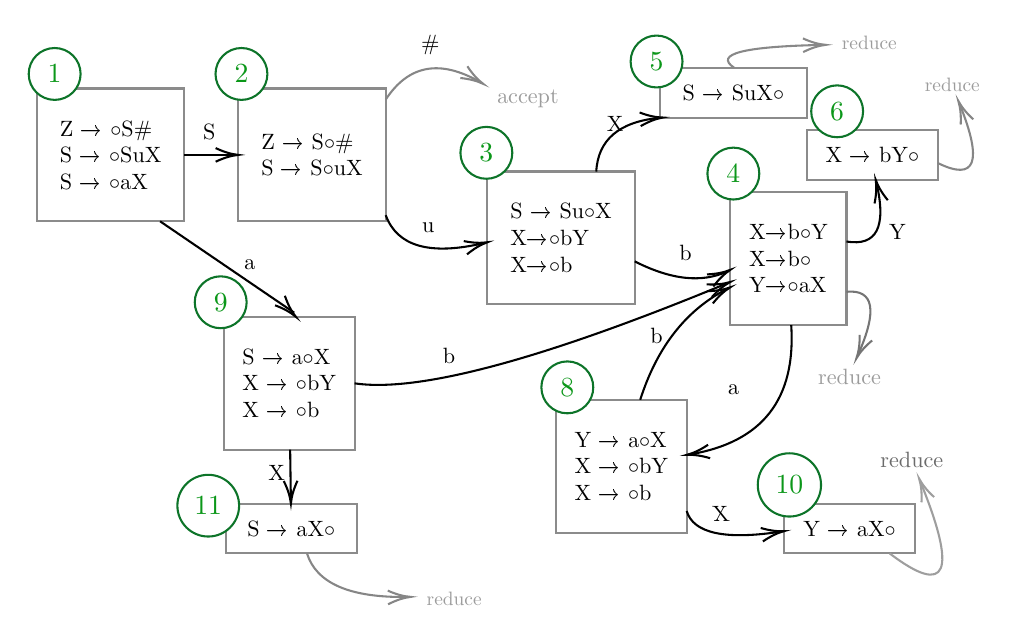
\begin{tikzpicture}[x=0.75pt,y=0.75pt,yscale=-1,xscale=1]
%uncomment if require: \path (0,283); %set diagram left start at 0, and has height of 283


% Text Node
\draw  [color={rgb, 255:red, 139; green, 139; blue, 139 }  ,draw opacity=1 ]  (8,28) -- (79,28) -- (79,92) -- (8,92) -- cycle  ;
\draw (43.5,60) node [scale=0.8,color={rgb, 255:red, 0; green, 0; blue, 0 }  ,opacity=1 ] [align=left] {Z → $\displaystyle \circ $S\#\\S → $\displaystyle \circ $SuX\\S → $\displaystyle \circ $aX};
% Text Node
\draw  [color={rgb, 255:red, 139; green, 139; blue, 139 }  ,draw opacity=1 ]  (105,28) -- (176,28) -- (176,92) -- (105,92) -- cycle  ;
\draw (140.5,60) node [scale=0.8,color={rgb, 255:red, 0; green, 0; blue, 0 }  ,opacity=1 ] [align=left] {Z → S$\displaystyle \circ $\#\\S → S$\displaystyle \circ $uX};
% Text Node
\draw  [color={rgb, 255:red, 139; green, 139; blue, 139 }  ,draw opacity=1 ]  (225,68) -- (296,68) -- (296,132) -- (225,132) -- cycle  ;
\draw (260.5,100) node [scale=0.8,color={rgb, 255:red, 0; green, 0; blue, 0 }  ,opacity=1 ] [align=left] {S → Su$\displaystyle \circ $X\\X→$\displaystyle \circ $bY\\X→$\displaystyle \circ $b};
% Text Node
\draw  [color={rgb, 255:red, 139; green, 139; blue, 139 }  ,draw opacity=1 ]  (342,78) -- (398,78) -- (398,142) -- (342,142) -- cycle  ;
\draw (370,110) node [scale=0.8,color={rgb, 255:red, 0; green, 0; blue, 0 }  ,opacity=1 ] [align=left] {X→b$\displaystyle \circ $Y\\X→b$\displaystyle \circ $\\Y→$\displaystyle \circ $aX};
% Text Node
\draw (244.5,33) node [scale=0.8,color={rgb, 255:red, 156; green, 156; blue, 156 }  ,opacity=1 ] [align=left] {accept};
% Text Node
\draw (91,49) node [scale=0.8] [align=left] {S};
% Text Node
\draw (197.5,7) node [scale=0.8] [align=left] {\#};
% Text Node
\draw (320.5,107) node [scale=0.8] [align=left] {b};
% Text Node
\draw (343.5,173) node [scale=0.8] [align=left] {a};
% Text Node
\draw (399.5,167) node [scale=0.8,color={rgb, 255:red, 156; green, 156; blue, 156 }  ,opacity=1 ] [align=left] {reduce};
% Text Node
\draw (337.5,233) node [scale=0.8,xslant=-0.14] [align=left] {X};
% Text Node
\draw (196.5,95) node [scale=0.8] [align=left] {u};
% Text Node
\draw  [color={rgb, 255:red, 139; green, 139; blue, 139 }  ,draw opacity=1 ]  (308,18) -- (379,18) -- (379,42) -- (308,42) -- cycle  ;
\draw (343.5,30) node [scale=0.8,color={rgb, 255:red, 0; green, 0; blue, 0 }  ,opacity=1 ] [align=left] {S → SuX$\displaystyle \circ $};
% Text Node
\draw (286.5,45) node [scale=0.8] [align=left] {X};
% Text Node
\draw  [color={rgb, 255:red, 139; green, 139; blue, 139 }  ,draw opacity=1 ]  (258,178) -- (321,178) -- (321,242) -- (258,242) -- cycle  ;
\draw (289.5,210) node [scale=0.8,color={rgb, 255:red, 0; green, 0; blue, 0 }  ,opacity=1 ] [align=left] {Y → a$\displaystyle \circ $X\\X → $\displaystyle \circ $bY\\X → $\displaystyle \circ $b};
% Text Node
\draw (306.5,147) node [scale=0.8] [align=left] {b};
% Text Node
\draw  [color={rgb, 255:red, 139; green, 139; blue, 139 }  ,draw opacity=1 ]  (379,48) -- (442,48) -- (442,72) -- (379,72) -- cycle  ;
\draw (410.5,60) node [scale=0.8,color={rgb, 255:red, 0; green, 0; blue, 0 }  ,opacity=1 ] [align=left] {X → bY$\displaystyle \circ $};
% Text Node
\draw (422.5,97) node [scale=0.8] [align=left] {Y};
% Text Node
\draw (449,26) node [scale=0.7,color={rgb, 255:red, 156; green, 156; blue, 156 }  ,opacity=1 ] [align=left] {reduce};
% Text Node
\draw  [color={rgb, 255:red, 139; green, 139; blue, 139 }  ,draw opacity=1 ]  (98,138) -- (161,138) -- (161,202) -- (98,202) -- cycle  ;
\draw (129.5,170) node [scale=0.8,color={rgb, 255:red, 0; green, 0; blue, 0 }  ,opacity=1 ] [align=left] {S → a$\displaystyle \circ $X\\X → $\displaystyle \circ $bY\\X → $\displaystyle \circ $b};
% Text Node
\draw (206.5,157) node [scale=0.8] [align=left] {b};
% Text Node
\draw (110.5,113) node [scale=0.8] [align=left] {a};
% Text Node
\draw  [color={rgb, 255:red, 139; green, 139; blue, 139 }  ,draw opacity=1 ]  (99,228) -- (162,228) -- (162,252) -- (99,252) -- cycle  ;
\draw (130.5,240) node [scale=0.8,color={rgb, 255:red, 0; green, 0; blue, 0 }  ,opacity=1 ] [align=left] {S → aX$\displaystyle \circ $};
% Text Node
\draw (209,274) node [scale=0.7,color={rgb, 255:red, 156; green, 156; blue, 156 }  ,opacity=1 ] [align=left] {reduce};
% Text Node
\draw (123.5,213) node [scale=0.8] [align=left] {X};
% Text Node
\draw  [color={rgb, 255:red, 139; green, 139; blue, 139 }  ,draw opacity=1 ]  (368,228) -- (431,228) -- (431,252) -- (368,252) -- cycle  ;
\draw (399.5,240) node [scale=0.8,color={rgb, 255:red, 0; green, 0; blue, 0 }  ,opacity=1 ] [align=left] {Y → aX$\displaystyle \circ $};
% Text Node
\draw (429.5,207) node [scale=0.8,color={rgb, 255:red, 107; green, 107; blue, 107 }  ,opacity=1 ] [align=left] {reduce};
% Text Node
\draw (409,6) node [scale=0.7,color={rgb, 255:red, 156; green, 156; blue, 156 }  ,opacity=1 ] [align=left] {reduce};
% Text Node
\draw  [color={rgb, 255:red, 13; green, 116; blue, 41 }  ,draw opacity=1 ][fill={rgb, 255:red, 255; green, 255; blue, 255 }  ,fill opacity=1 ]  (16.5, 21) circle [x radius= 12.5, y radius= 12.5]   ;
\draw (16.5,21) node [color={rgb, 255:red, 11; green, 151; blue, 25 }  ,opacity=1 ] [align=left] {1};
% Text Node
\draw  [color={rgb, 255:red, 13; green, 116; blue, 41 }  ,draw opacity=1 ][fill={rgb, 255:red, 255; green, 255; blue, 255 }  ,fill opacity=1 ]  (106.5, 21) circle [x radius= 12.5, y radius= 12.5]   ;
\draw (106.5,21) node [color={rgb, 255:red, 11; green, 151; blue, 25 }  ,opacity=1 ] [align=left] {2};
% Text Node
\draw  [color={rgb, 255:red, 13; green, 116; blue, 41 }  ,draw opacity=1 ][fill={rgb, 255:red, 255; green, 255; blue, 255 }  ,fill opacity=1 ]  (224.5, 59) circle [x radius= 12.5, y radius= 12.5]   ;
\draw (224.5,59) node [color={rgb, 255:red, 11; green, 151; blue, 25 }  ,opacity=1 ] [align=left] {3};
% Text Node
\draw  [color={rgb, 255:red, 13; green, 116; blue, 41 }  ,draw opacity=1 ][fill={rgb, 255:red, 255; green, 255; blue, 255 }  ,fill opacity=1 ]  (343.5, 69) circle [x radius= 12.5, y radius= 12.5]   ;
\draw (343.5,69) node [color={rgb, 255:red, 11; green, 151; blue, 25 }  ,opacity=1 ] [align=left] {4};
% Text Node
\draw  [color={rgb, 255:red, 13; green, 116; blue, 41 }  ,draw opacity=1 ][fill={rgb, 255:red, 255; green, 255; blue, 255 }  ,fill opacity=1 ]  (306.5, 15) circle [x radius= 12.5, y radius= 12.5]   ;
\draw (306.5,15) node [color={rgb, 255:red, 11; green, 151; blue, 25 }  ,opacity=1 ] [align=left] {5};
% Text Node
\draw  [color={rgb, 255:red, 13; green, 116; blue, 41 }  ,draw opacity=1 ][fill={rgb, 255:red, 255; green, 255; blue, 255 }  ,fill opacity=1 ]  (393.5, 39) circle [x radius= 12.5, y radius= 12.5]   ;
\draw (393.5,39) node [color={rgb, 255:red, 11; green, 151; blue, 25 }  ,opacity=1 ] [align=left] {6};
% Text Node
\draw  [color={rgb, 255:red, 13; green, 116; blue, 41 }  ,draw opacity=1 ][fill={rgb, 255:red, 255; green, 255; blue, 255 }  ,fill opacity=1 ]  (263.5, 172) circle [x radius= 12.5, y radius= 12.5]   ;
\draw (263.5,172) node [color={rgb, 255:red, 11; green, 151; blue, 25 }  ,opacity=1 ] [align=left] {8};
% Text Node
\draw  [color={rgb, 255:red, 13; green, 116; blue, 41 }  ,draw opacity=1 ][fill={rgb, 255:red, 255; green, 255; blue, 255 }  ,fill opacity=1 ]  (96.5, 131) circle [x radius= 12.5, y radius= 12.5]   ;
\draw (96.5,131) node [color={rgb, 255:red, 11; green, 151; blue, 25 }  ,opacity=1 ] [align=left] {9};
% Text Node
\draw  [color={rgb, 255:red, 13; green, 116; blue, 41 }  ,draw opacity=1 ][fill={rgb, 255:red, 255; green, 255; blue, 255 }  ,fill opacity=1 ]  (370.5, 219) circle [x radius= 15.24, y radius= 15.24]   ;
\draw (370.5,219) node [color={rgb, 255:red, 11; green, 151; blue, 25 }  ,opacity=1 ] [align=left] {10};
% Text Node
\draw  [color={rgb, 255:red, 13; green, 116; blue, 41 }  ,draw opacity=1 ][fill={rgb, 255:red, 255; green, 255; blue, 255 }  ,fill opacity=1 ]  (90.5, 229) circle [x radius= 14.87, y radius= 14.87]   ;
\draw (90.5,229) node [color={rgb, 255:red, 11; green, 151; blue, 25 }  ,opacity=1 ] [align=left] {11};
% Connection
\draw    (79,60) -- (103,60) ;
\draw [shift={(105,60)}, rotate = 180] [color={rgb, 255:red, 0; green, 0; blue, 0 }  ][line width=0.75]    (10.93,-3.29) .. controls (6.95,-1.4) and (3.31,-0.3) .. (0,0) .. controls (3.31,0.3) and (6.95,1.4) .. (10.93,3.29)   ;

% Connection
\draw    (176,89.04) .. controls (181.56,104.13) and (197.36,108.61) .. (223.39,102.47) ;
\draw [shift={(225,102.08)}, rotate = 526.04] [color={rgb, 255:red, 0; green, 0; blue, 0 }  ][line width=0.75]    (10.93,-3.29) .. controls (6.95,-1.4) and (3.31,-0.3) .. (0,0) .. controls (3.31,0.3) and (6.95,1.4) .. (10.93,3.29)   ;

% Connection
\draw    (296,111.32) .. controls (313.43,120.16) and (328.19,121.8) .. (340.31,116.23) ;
\draw [shift={(342,115.39)}, rotate = 512.21] [color={rgb, 255:red, 0; green, 0; blue, 0 }  ][line width=0.75]    (10.93,-3.29) .. controls (6.95,-1.4) and (3.31,-0.3) .. (0,0) .. controls (3.31,0.3) and (6.95,1.4) .. (10.93,3.29)   ;

% Connection
\draw [color={rgb, 255:red, 134; green, 134; blue, 134 }  ,draw opacity=1 ]   (176,33.36) .. controls (186.96,16.6) and (202.13,13.79) .. (221.5,24.91) ;
\draw [shift={(223,25.79)}, rotate = 211.15] [color={rgb, 255:red, 134; green, 134; blue, 134 }  ,draw opacity=1 ][line width=0.75]    (10.93,-3.29) .. controls (6.95,-1.4) and (3.31,-0.3) .. (0,0) .. controls (3.31,0.3) and (6.95,1.4) .. (10.93,3.29)   ;

% Connection
\draw [color={rgb, 255:red, 117; green, 117; blue, 117 }  ,draw opacity=1 ]   (398,125.95) .. controls (411.22,124.71) and (413.07,134.83) .. (403.56,156.32) ;
\draw [shift={(402.8,158)}, rotate = 294.58] [color={rgb, 255:red, 117; green, 117; blue, 117 }  ,draw opacity=1 ][line width=0.75]    (10.93,-3.29) .. controls (6.95,-1.4) and (3.31,-0.3) .. (0,0) .. controls (3.31,0.3) and (6.95,1.4) .. (10.93,3.29)   ;

% Connection
\draw    (277.44,68) .. controls (278.29,52.74) and (288.38,44.13) .. (307.69,42.16) ;
\draw [shift={(309.5,42)}, rotate = 535.54] [color={rgb, 255:red, 0; green, 0; blue, 0 }  ][line width=0.75]    (10.93,-3.29) .. controls (6.95,-1.4) and (3.31,-0.3) .. (0,0) .. controls (3.31,0.3) and (6.95,1.4) .. (10.93,3.29)   ;

% Connection
\draw    (371.37,142) .. controls (373.69,177.69) and (357.44,198.45) .. (322.6,204.28) ;
\draw [shift={(321,204.53)}, rotate = 351.37] [color={rgb, 255:red, 0; green, 0; blue, 0 }  ][line width=0.75]    (10.93,-3.29) .. controls (6.95,-1.4) and (3.31,-0.3) .. (0,0) .. controls (3.31,0.3) and (6.95,1.4) .. (10.93,3.29)   ;

% Connection
\draw    (298.62,178) .. controls (306.74,152.56) and (320.69,134.76) .. (340.47,124.57) ;
\draw [shift={(342,123.8)}, rotate = 513.98] [color={rgb, 255:red, 0; green, 0; blue, 0 }  ][line width=0.75]    (10.93,-3.29) .. controls (6.95,-1.4) and (3.31,-0.3) .. (0,0) .. controls (3.31,0.3) and (6.95,1.4) .. (10.93,3.29)   ;

% Connection
\draw    (398,101.72) .. controls (412.54,104.14) and (417.36,94.78) .. (412.48,73.65) ;
\draw [shift={(412.08,72)}, rotate = 436.1] [color={rgb, 255:red, 0; green, 0; blue, 0 }  ][line width=0.75]    (10.93,-3.29) .. controls (6.95,-1.4) and (3.31,-0.3) .. (0,0) .. controls (3.31,0.3) and (6.95,1.4) .. (10.93,3.29)   ;

% Connection
\draw [color={rgb, 255:red, 134; green, 134; blue, 134 }  ,draw opacity=1 ]   (442,63.91) .. controls (460.24,72.88) and (463.76,63.48) .. (452.59,35.72) ;
\draw [shift={(451.89,34)}, rotate = 427.56] [color={rgb, 255:red, 134; green, 134; blue, 134 }  ,draw opacity=1 ][line width=0.75]    (10.93,-3.29) .. controls (6.95,-1.4) and (3.31,-0.3) .. (0,0) .. controls (3.31,0.3) and (6.95,1.4) .. (10.93,3.29)   ;

% Connection
\draw    (67.3,92) -- (131.9,136.01) ;
\draw [shift={(132.7,138)}, rotate = 225.71] [color={rgb, 255:red, 0; green, 0; blue, 0 }  ][line width=0.75]    (10.93,-3.29) .. controls (6.95,-1.4) and (3.31,-0.3) .. (0,0) .. controls (3.31,0.3) and (6.95,1.4) .. (10.93,3.29)   ;

% Connection
\draw    (161,170.06) .. controls (191.85,174.63) and (251.75,158.53) .. (340.66,121.79) ;
\draw [shift={(342,121.23)}, rotate = 517.5] [color={rgb, 255:red, 0; green, 0; blue, 0 }  ][line width=0.75]    (10.93,-3.29) .. controls (6.95,-1.4) and (3.31,-0.3) .. (0,0) .. controls (3.31,0.3) and (6.95,1.4) .. (10.93,3.29)   ;

% Connection
\draw    (129.96,202) -- (130.3,226) ;
\draw [shift={(130.33,228)}, rotate = 269.18] [color={rgb, 255:red, 0; green, 0; blue, 0 }  ][line width=0.75]    (10.93,-3.29) .. controls (6.95,-1.4) and (3.31,-0.3) .. (0,0) .. controls (3.31,0.3) and (6.95,1.4) .. (10.93,3.29)   ;

% Connection
\draw [color={rgb, 255:red, 134; green, 134; blue, 134 }  ,draw opacity=1 ]   (138.07,252) .. controls (142.6,266.38) and (158.67,273.37) .. (186.29,272.98) ;
\draw [shift={(188,272.95)}, rotate = 538.5899999999999] [color={rgb, 255:red, 134; green, 134; blue, 134 }  ,draw opacity=1 ][line width=0.75]    (10.93,-3.29) .. controls (6.95,-1.4) and (3.31,-0.3) .. (0,0) .. controls (3.31,0.3) and (6.95,1.4) .. (10.93,3.29)   ;

% Connection
\draw    (321,231.58) .. controls (324.26,242.31) and (339.38,245.62) .. (366.33,241.52) ;
\draw [shift={(368,241.26)}, rotate = 530.89] [color={rgb, 255:red, 0; green, 0; blue, 0 }  ][line width=0.75]    (10.93,-3.29) .. controls (6.95,-1.4) and (3.31,-0.3) .. (0,0) .. controls (3.31,0.3) and (6.95,1.4) .. (10.93,3.29)   ;

% Connection
\draw [color={rgb, 255:red, 158; green, 158; blue, 158 }  ,draw opacity=1 ]   (418.79,252) .. controls (446.65,273.12) and (451.57,261.57) .. (433.57,217.35) ;
\draw [shift={(433.02,216)}, rotate = 427.63] [color={rgb, 255:red, 158; green, 158; blue, 158 }  ,draw opacity=1 ][line width=0.75]    (10.93,-3.29) .. controls (6.95,-1.4) and (3.31,-0.3) .. (0,0) .. controls (3.31,0.3) and (6.95,1.4) .. (10.93,3.29)   ;

% Connection
\draw [color={rgb, 255:red, 136; green, 136; blue, 136 }  ,draw opacity=1 ]   (343.86,18) .. controls (334.1,11.43) and (348.23,7.77) .. (386.25,7.02) ;
\draw [shift={(388,6.98)}, rotate = 539.01] [color={rgb, 255:red, 136; green, 136; blue, 136 }  ,draw opacity=1 ][line width=0.75]    (10.93,-3.29) .. controls (6.95,-1.4) and (3.31,-0.3) .. (0,0) .. controls (3.31,0.3) and (6.95,1.4) .. (10.93,3.29)   ;


\end{tikzpicture}

